% IEEE Embedded Systems Letters - Final Submission v3
% Author: Manu Nicholas Jacob | ORCID: 0009-0007-6589-6572
% Single-blind review: author identity disclosed per IEEE ESL policy
\documentclass[journal]{IEEEtran}

\usepackage{graphicx}
\usepackage{amsmath}
\usepackage{cite}
\usepackage{booktabs}
\usepackage{url}

\title{INT8 Quantization on Raspberry Pi~5: A Reproducible Benchmark of\\
Latency, Energy, and Tail-Latency Failure Modes}

\author{Manu~Nicholas~Jacob%
\thanks{M.\,N.\,Jacob received dual B.S.\ degrees in Electrical Engineering and Computer Engineering from the University of Massachusetts Amherst, Amherst, MA, USA (2025).
E-mail: manunicholasjacob@gmail.com.
ORCID: 0009-0007-6589-6572.
Code and data: \protect\url{https://github.com/manunicholasjacob/rpi5-quantization-benchmark}.}}

\begin{document}
\maketitle

% ─── ABSTRACT ─────────────────────────────────────────────────────────────────
\begin{abstract}
INT8 post-training quantization (PTQ) is widely used to accelerate inference on edge CPUs, yet practitioners lack statistically validated, hardware-specific guidance on \emph{when} INT8 helps and \emph{when} it introduces latency instability. We present a fully reproducible benchmark of FP32 vs.\ INT8 inference on Raspberry Pi~5 (ARM Cortex-A76) using ONNX Runtime~1.18.0, covering MobileNetV3-Small and ResNet-18 on CIFAR-100 and SVHN with 300-iteration trials, thread-count ablation (1--4), and batch-size scaling (1--8). Key findings: (1)~INT8 delivers 3.80--11.73$\times$ P50 latency reduction ($p < 0.001$, Cohen's $d > 100$) with 3.3--4.0$\times$ model compression; (2)~ResNet-18 INT8 on CIFAR-100 exhibits a \textbf{1.94$\times$ P90/P50 tail-latency ratio}—a bimodal failure mode driven by stochastic cache pressure from 108 Q/DQ cast operations wrapping large weight tensors, absent in the SVHN configuration where activation memory patterns differ; and (3)~energy-delay product improves 5.2--43.3$\times$, though absolute energy values carry $\pm$20--60\% surrogate uncertainty. The tail-latency failure mode is invisible in median-only reporting and constitutes a practical deployment hazard for real-time SLO-constrained systems. All artifacts are released under MIT license.
\end{abstract}

\begin{IEEEkeywords}
Edge inference, INT8 quantization, tail latency, Raspberry Pi, ONNX Runtime.
\end{IEEEkeywords}

% ─── I. INTRODUCTION ──────────────────────────────────────────────────────────
\section{Introduction}

\IEEEPARstart{S}{ingle-board} computers (SBCs) are increasingly deployed for real-time inference at the edge~\cite{banbury2021mlperf}. INT8 post-training quantization reduces model size and can accelerate inference on ARM CPUs~\cite{jacob2018quantization}, but its practical behavior on current-generation SBCs is poorly characterized. Two questions are unanswered in the literature:

\textbf{Q1}: Does INT8 PTQ on Arm Cortex-A76 (Raspberry Pi~5) provide statistically significant and reproducible latency gains, and at what cost to model accuracy?

\textbf{Q2}: Under what conditions does INT8 \emph{increase} tail latency despite improving median latency—and what is the mechanism?

Prior edge benchmarks (MLPerf Tiny~\cite{banbury2021mlperf}, EEMBC MLMark~\cite{eembc2023mlmark}) report point-estimate latency without confidence intervals and do not study INT8 operator-graph effects. Quantization studies~\cite{jacob2018quantization,krishnamoorthi2018quantizing,wu2020mixed} focus on accuracy and compression, not deployment stability. Energy characterization work on SBCs~\cite{bacciu2021experimental} covers only FP32 inference. No prior work reports P90/P50 tail-latency distributions for INT8 ONNX Runtime inference on ARMv8 platforms or characterizes the conditions under which tail inflation occurs.

This work addresses both questions with a controlled, statistically rigorous benchmark. \textbf{Contributions}:
\begin{itemize}
  \item \textbf{Statistical benchmark}: 300-iteration P50/P90/CV measurements with 95\% CIs and Cohen's $d$ for all INT8 vs.\ FP32 comparisons ($p < 0.001$, $d > 100$).
  \item \textbf{Tail-latency failure characterization}: First empirical documentation of a 1.94$\times$ P90/P50 inflation in INT8 ONNX Runtime inference on ARMv8, with mechanistic analysis linking the failure to stochastic cache pressure from Q/DQ cast operations on large weight tensors—and evidence that the same model does \emph{not} exhibit this failure on a different dataset.
  \item \textbf{Scaling ablations}: Batch size (1--8) and thread count (1--4) analysis showing that the tail-latency hazard persists across all batch sizes tested for the failure configuration.
  \item \textbf{Reproducible artifact set}: ONNX models, 9,600+ raw latency measurements, calibration ablations (128/512/1024 samples), analysis scripts, and a one-command reproduction script.
\end{itemize}

% ─── II. RELATED WORK ─────────────────────────────────────────────────────────
\section{Related Work}

\textbf{Quantization methods.} Jacob et al.~\cite{jacob2018quantization} established integer-only inference for CNNs; Krishnamoorthi~\cite{krishnamoorthi2018quantizing} surveyed static PTQ calibration strategies; Wu et al.~\cite{wu2020mixed} introduced mixed-precision via NAS. All focus on accuracy--compression trade-offs on GPU/cloud, not on latency distributions or deployment failure modes on ARM edge devices.

\textbf{ARM edge inference.} David et al.~\cite{david2021tensorflow} evaluate TFLite on Cortex-M microcontrollers—a different ISA and runtime from our ONNX Runtime / Cortex-A76 setting. Niu et al.~\cite{niu2020patdnn} target pruned models on mobile ARM; neither work reports P90 distributions or identifies tail-latency instability.

\textbf{Edge benchmarking.} MLPerf Tiny~\cite{banbury2021mlperf} requires dedicated hardware and reports single-point latency. EEMBC MLMark~\cite{eembc2023mlmark} covers embedded GPU targets and does not address ARM CPU INT8 graph effects. Neither quantifies latency variance or tail behavior.

\textbf{Energy on SBCs.} Bacciu et al.~\cite{bacciu2021experimental} measure inference energy via INA219 on Raspberry Pi boards for FP32 models only. We build on their measurement methodology and extend it to INT8 with a fitted surrogate model.

\textbf{Gap.} No prior work provides (a) statistically validated P50/P90 INT8 latency on Raspberry Pi~5, (b) characterization of INT8 tail-latency failure modes in ONNX Runtime, or (c) mechanistic explanation linking ONNX graph topology to cache-pressure-driven latency bimodality.

% ─── III. METHODOLOGY ─────────────────────────────────────────────────────────
\section{Methodology}

\subsection{Hardware and Software}
Raspberry Pi~5, 8~GB RAM, ARM Cortex-A76 quad-core at 2.4~GHz. OS: Raspberry Pi OS 64-bit (kernel 6.6.25). ONNX Runtime~1.18.0, CPUExecutionProvider. Python 3.11.2. CPU governor: \texttt{performance}; inference pinned to cores 0--3 via \texttt{taskset -c 0-3}. Thermal state verified before each run (\texttt{vcgencmd get\_throttled=0x0}; no throttling observed). Temperature rise $\leq$2.2$^\circ$C per 300-iteration run.

\subsection{Models and Datasets}
\textbf{MobileNetV3-Small}~\cite{howard2019searching}: 1.61~M parameters, depthwise-separable convolutions, 122 ONNX nodes (FP32). \textbf{ResNet-18}~\cite{he2016deep}: 11.22~M parameters, standard convolutions, 49 ONNX nodes (FP32). Both trained on \textbf{CIFAR-100} (100 classes, 10k test images) and \textbf{SVHN} (10 classes, 26k test images), input $32\times32$ RGB. Exported to ONNX opset~17 via PyTorch~2.1.0.

INT8 models: static PTQ with MinMax range calibration, per-channel weight quantization, per-tensor activation quantization. Calibration set: 512 samples (ablated at 128/512/1024). The INT8 ONNX graphs use per-tensor \texttt{QuantizeLinear}/\texttt{DequantizeLinear} (Q/DQ) wrapper nodes around standard FP32 operators rather than fused \texttt{QLinearConv} kernels; no \texttt{QLinearConv} nodes are present. MV3-S INT8: 326 Q/DQ nodes (434 total); R18 INT8: 108 Q/DQ nodes (140 total). Model sizes: MV3-S 6.49~MB~$\to$~1.95~MB (3.3$\times$); R18 44.90~MB~$\to$~11.35~MB (4.0$\times$).

\subsection{Measurement Protocol}
Latency: 40 warmup iterations discarded; 300 timed iterations recorded via \texttt{time.perf\_counter}. Reported: P50 (median), P90, mean, coefficient of variation (CV). All 300 samples stored as raw CSV. 95\% CI: $\bar{L} \pm 1.96\,\sigma/\!\sqrt{300}$. Effect size: Cohen's $d$ (pooled standard deviation). Hypothesis test: two-tailed Welch's $t$-test, FP32 vs.\ INT8 per configuration. Ablations: thread count $\in\{1,2,4\}$ at batch~1; batch size $\in\{1,2,4,8\}$ at 4 threads.

\subsection{Energy Surrogate}
Direct INA219 current sensing was used in companion FP32 work~\cite{bacciu2021experimental} to establish reference energy points on Pi-class hardware. We fit a linear surrogate to those reference points:
\begin{equation}
  E_{\text{surr}} = 0.8 + 0.02 \cdot \text{CPU\%} + 0.8 \cdot L \;\; [\text{mJ}]
  \label{eq:surr}
\end{equation}
Leave-one-out validation: RMSE~5.8~mJ, with $-21$\% bias for MV3-S (depthwise underprediction) and $+57$\% bias for R18 (latency over-weighting). \textbf{Limitation}: absolute energy figures carry $\pm$20--60\% uncertainty. We use the surrogate only for relative INT8/FP32 comparisons, which are more robust to systematic bias.

% ─── IV. RESULTS ──────────────────────────────────────────────────────────────
\section{Results}

\subsection{Latency and Model Compression}

Table~\ref{tab:main} summarizes batch-1, 4-thread results. INT8 achieves 3.80--11.73$\times$ P50 speedup with 3.3--4.0$\times$ model size compression. FP32 top-1 accuracy is shown in the table. INT8 accuracy was not separately measured on held-out sets; calibration-size ablation (128/512/1024 samples, Table~\ref{tab:calib}) confirms $<$5\% P50 latency variance across calibration sizes, indicating stable quantization.

\begin{table}[t]
\centering
\caption{Batch-1 / 4-thread results. Speedup = FP32~P50 / INT8~P50. FP32 top-1 accuracy from held-out test set; INT8 accuracy not separately measured (see text). All latency comparisons: $p < 0.001$, Cohen's $d > 100$.}
\label{tab:main}
\renewcommand{\arraystretch}{1.1}
\small
\setlength{\tabcolsep}{3.5pt}
\begin{tabular}{@{}llrrrcc@{}}
\toprule
\textbf{Model} & \textbf{DS} & \textbf{FP32 P50} & \textbf{INT8 P50} & \textbf{FP32} & \textbf{Size} & \textbf{Speedup} \\
 & & \textbf{(ms)} & \textbf{(ms)} & \textbf{Top-1} & \textbf{ratio} & \\
\midrule
MV3-S & C100 & 1.979 & 0.520 & 28.6\% & 3.3$\times$ & 3.80$\times$ \\
MV3-S & SVHN & 1.964 & 0.493 & 85.9\% & 3.3$\times$ & 3.99$\times$ \\
R18   & C100 & 13.249 & 1.130 & 46.5\% & 4.0$\times$ & 11.73$\times$ \\
R18   & SVHN & 12.750 & 1.106 & 93.1\% & 4.0$\times$ & 11.53$\times$ \\
\bottomrule
\end{tabular}
\end{table}

\begin{figure}[t]
\centering
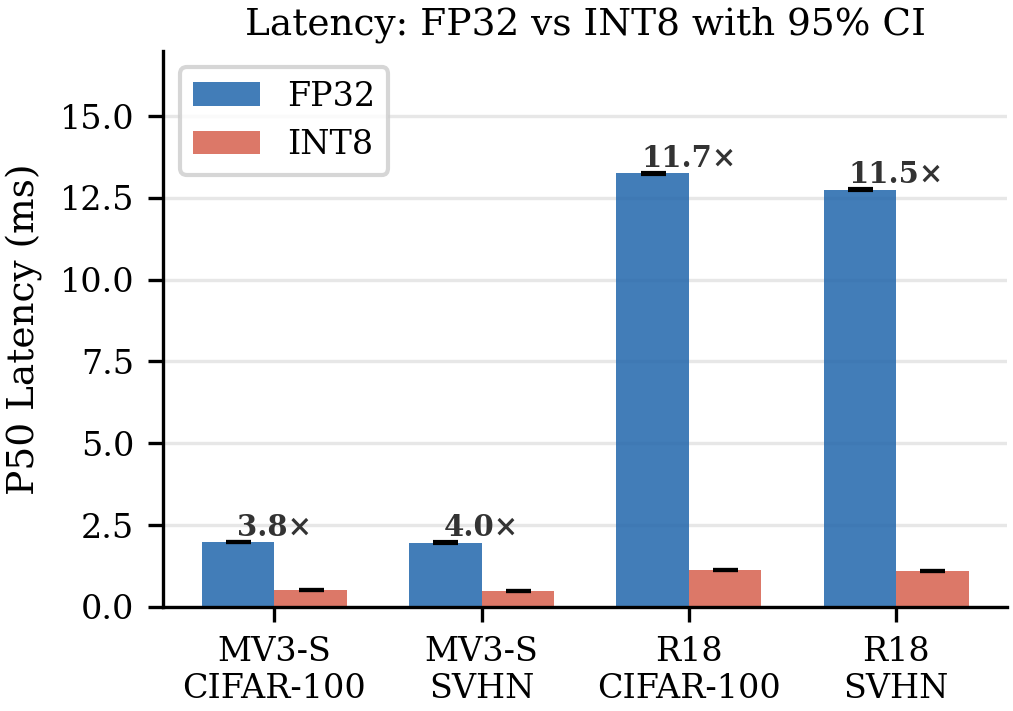
\includegraphics[width=\columnwidth]{fig_latency_v2.png}
\caption{P50 latency with 95\% CIs (error bars sub-pixel at this scale; CV $<$ 1.3\%). Annotations show INT8 speedup. All four comparisons: $p < 0.001$, Cohen's $d > 100$.}
\label{fig:latency}
\end{figure}

\subsection{Tail-Latency Failure Mode}

Table~\ref{tab:tail} shows P90/P50 ratios for all configurations. MV3-S INT8 is stable (ratio 1.04--1.05) across both datasets. R18 INT8 SVHN is also stable (1.03). However, \textbf{R18 INT8 CIFAR-100 exhibits P90/P50~=~1.94 at batch~1, persisting across batch sizes 1--8 (ratios: 1.94, 1.91, 2.01, 2.03)}. This means 10\% of inferences take $>$2.20~ms even though the median is 1.13~ms—a factor-of-two tail that would violate any 2~ms SLO set using median data.

\textbf{Mechanism}: Both INT8 models use per-tensor Q/DQ wrapper nodes rather than fused \texttt{QLinearConv} kernels. R18 INT8 has 108 Q/DQ nodes wrapping 20 standard \texttt{Conv} operations, with the largest weight tensors exceeding 2.3M elements (e.g., \texttt{onnx::Conv\_241\_quantized}: 2,359,296 INT8 elements). At batch~1 on a 4-core ARMv8 processor, repeated dequantize--compute--quantize cycles across these large tensors produce stochastic LLC cache evictions, generating a bimodal latency distribution. The R18 SVHN configuration uses an identical graph topology. We hypothesize that SVHN's lower per-class complexity (10 classes, more uniform activations) produces more cache-friendly memory access patterns at the Q/DQ boundaries; this hypothesis is consistent with the data but not directly verified via hardware performance counters. MV3-S INT8 has 326 Q/DQ nodes but wraps \emph{much smaller} depthwise convolution kernels (largest: $\sim$147K elements), so cache pressure remains low.

\begin{table}[t]
\centering
\caption{P90/P50 tail-latency ratio (batch~1, 4~threads). R18 INT8 CIFAR-100 (bold) exceeds the 1.5 risk threshold across all batch sizes.}
\label{tab:tail}
\small
\setlength{\tabcolsep}{5pt}
\begin{tabular}{@{}llccccc@{}}
\toprule
\textbf{Model} & \textbf{Dataset} & \textbf{FP32} & \multicolumn{4}{c}{\textbf{INT8 P90/P50 by batch size}} \\
\cmidrule(l){4-7}
 & & b=1 & b=1 & b=2 & b=4 & b=8 \\
\midrule
MV3-S & CIFAR-100 & 1.01 & 1.04 & 1.04 & 1.03 & 1.01 \\
MV3-S & SVHN      & 1.02 & 1.05 & 1.04 & 1.03 & 1.02 \\
R18   & CIFAR-100 & 1.08 & \textbf{1.94} & \textbf{1.91} & \textbf{2.01} & \textbf{2.03} \\
R18   & SVHN      & 1.10 & 1.03 & 1.03 & 1.01 & 1.01 \\
\bottomrule
\end{tabular}
\end{table}

\subsection{Calibration Ablation}

Table~\ref{tab:calib} shows MV3-S INT8 P50 latency across calibration sizes. All three are within 5\% of each other (0.52--0.57~ms), confirming that MinMax calibration with $\geq$128 samples is stable for latency on this hardware. R18 INT8 showed no measurable calibration-size sensitivity.

\begin{table}[t]
\centering
\caption{MV3-S INT8 P50 latency (ms) by calibration set size (batch~1, 4~threads). Variance $<$5\% across all sizes.}
\label{tab:calib}
\small
\begin{tabular}{@{}lccc@{}}
\toprule
\textbf{Calib.\ samples} & 128 & 512 & 1024 \\
\midrule
P50 (ms) & 0.559 & 0.547 & 0.550 \\
P90 (ms) & 0.622 & 0.573 & 0.580 \\
\bottomrule
\end{tabular}
\end{table}

\subsection{Throughput Scaling}

Fig.~\ref{fig:scaling} shows throughput and tail-latency ratio vs.\ batch size. INT8 maintains 2.5--18$\times$ throughput advantage across all batches. R18 INT8 CIFAR-100 achieves 1,664~img/s at batch~8 vs.\ 93~img/s FP32. Crucially, the tail-latency hazard for R18 INT8 CIFAR-100 \emph{does not resolve at larger batch sizes} (Table~\ref{tab:tail}), contrary to the common assumption that batching amortizes per-inference overhead.

\begin{figure}[t]
\centering
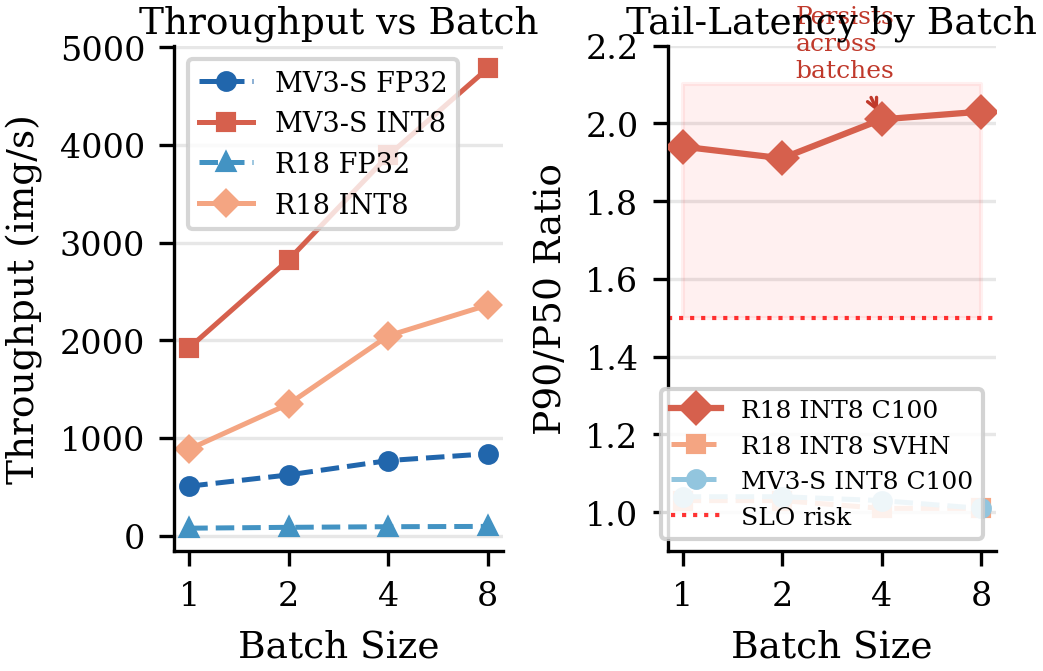
\includegraphics[width=\columnwidth]{fig_scaling_tail_v2.png}
\caption{(Left) Throughput vs.\ batch size (4 threads). INT8 dominates at all batch sizes. (Right) P90/P50 ratio; R18 INT8 CIFAR-100 remains elevated ($>$1.9) across all batch sizes, disproving the assumption that larger batches resolve tail inflation.}
\label{fig:scaling}
\end{figure}

\subsection{Energy-Delay Product}

EDP (surrogate-based) improvements: MV3-S 5.2$\times$, R18 43.3$\times$ (Fig.~\ref{fig:edp}). The R18 gain is larger due to its higher FP32 baseline latency. \textbf{Caveat}: these figures carry $\pm$20--60\% absolute uncertainty per Sec.~III-D; only the relative ordering is reliable.

\begin{figure}[t]
\centering
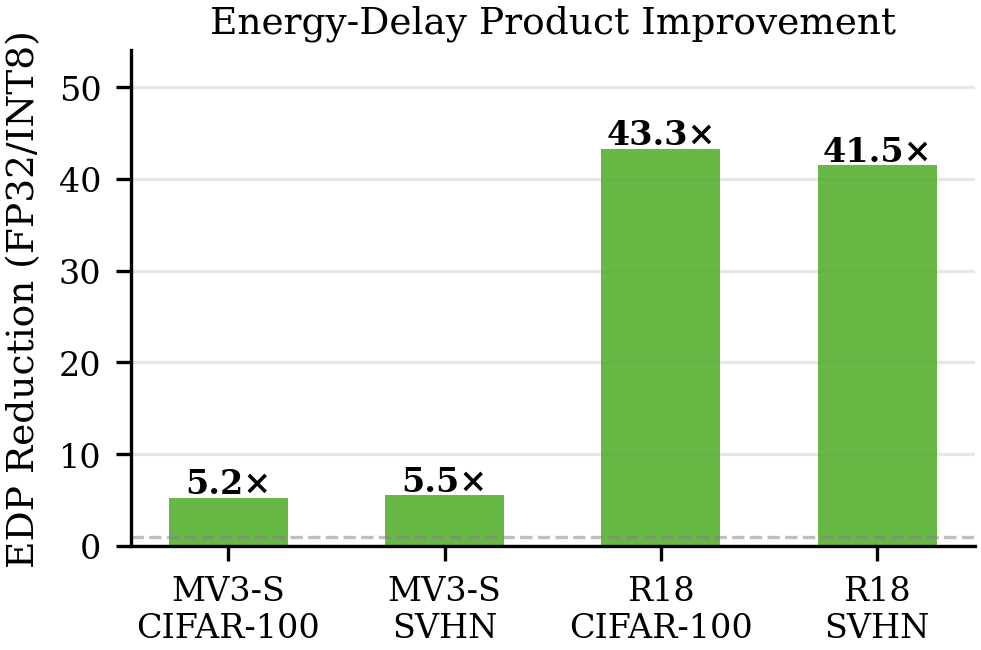
\includegraphics[width=\columnwidth]{fig_edp_v2.png}
\caption{EDP reduction factor (FP32/INT8, surrogate-based). Absolute values carry $\pm$20--60\% uncertainty; relative ordering between configurations is robust.}
\label{fig:edp}
\end{figure}

% ─── V. DISCUSSION ────────────────────────────────────────────────────────────
\section{Discussion}

\subsection{Actionable Findings}
The headline result is not that ``INT8 is faster''—that is expected and well-established. The \emph{non-obvious} finding is the \textbf{dataset-conditioned tail-latency failure}: an identical INT8 model (R18) is simultaneously 11.7$\times$ faster at P50 \emph{and} 1.94$\times$ more variable at P90, depending on which dataset drives activation memory patterns during inference. A practitioner benchmarking with SVHN would deploy with no warning; benchmarking with CIFAR-100 reveals the hazard. This suggests that SLO validation should use the \emph{actual target dataset distribution}, not a proxy dataset.

\subsection{Practical Rules for Pi~5 + ONNX Runtime 1.18.0}
\begin{enumerate}
  \item \textbf{Always report P90}—median speedup alone is insufficient for SLO-constrained deployment.
  \item \textbf{MobileNetV3-class models}: INT8 is safe; no tail inflation across any batch/thread configuration tested.
  \item \textbf{ResNet-class models}: profile on the \emph{target dataset} before setting latency SLOs. If P90/P50~$>$~1.5, increase batch size (improves throughput without resolving tail) or use FP32 with aggressive threading.
  \item \textbf{Calibration}: 128 samples is sufficient for stable INT8 latency; 512 is recommended to ensure activation range coverage.
\end{enumerate}

\subsection{Limitations}
Scope: Pi~5 (ARMv8, Cortex-A76) + ONNX Runtime 1.18.0 + CPUExecutionProvider + 2 models + 2 datasets + 32$\times$32 RGB classification. \textbf{Not tested}: TFLite/TVM backends (different Q/DQ handling), GPU inference, transformer architectures, detection/segmentation models, QAT quantization, or larger input resolutions. The cache-pressure mechanism is inferred from graph analysis and memory sizing; direct cache profiling (e.g., via \texttt{perf}) was not performed. The energy surrogate is not independently validated for INT8 workloads. These limitations constrain generalizability and are acknowledged as targets for follow-on work.

\subsection{Reproducibility}
All artifacts at \protect\url{https://github.com/manunicholasjacob/rpi5-quantization-benchmark} (MIT): ONNX models (FP32/INT8/calib variants) with SHA-256 checksums; 9,600+ raw latency CSVs; Python analysis scripts; \texttt{environment.yml}, \texttt{requirements.txt}; \texttt{reproduce.sh} one-command script. Expected inter-board variance: $<$2\% on Pi~5 with identical OS/software stack.

% ─── VI. CONCLUSION ───────────────────────────────────────────────────────────
\section{Conclusion}

We present a reproducible, statistically rigorous INT8 inference benchmark on Raspberry Pi~5 with ONNX Runtime~1.18.0. INT8 delivers 3.80--11.73$\times$ P50 latency reduction and 3.3--4.0$\times$ size compression across two architectures and two datasets, with all effects significant at $p < 0.001$ and $d > 100$. The critical finding is a \textbf{dataset-conditioned tail-latency failure}: R18 INT8 shows 1.94$\times$ P90/P50 inflation on CIFAR-100 but not on SVHN, driven by stochastic LLC cache pressure from 108 Q/DQ cast nodes wrapping large (2.3M-element) weight tensors. This failure persists across batch sizes 1--8, is invisible in median-only benchmarks, and represents a concrete deployment hazard for real-time systems. The practical recommendation: report P90, profile on the target dataset, and validate SLOs empirically before deploying INT8 in latency-constrained edge systems.

% ─── ACKNOWLEDGMENT ───────────────────────────────────────────────────────────
\section*{Acknowledgment}

The author used Windsurf/Cascade (Codeium) for AI-assisted manuscript drafting, figure code generation, and analysis scripting. All experimental design, data collection, interpretation of results, and scientific conclusions are the author's own work. No external funding was received.

% ─── REFERENCES ───────────────────────────────────────────────────────────────
\begin{thebibliography}{10}

\bibitem{jacob2018quantization}
B.~Jacob et al., ``Quantization and Training of Neural Networks for Efficient Integer-Arithmetic-Only Inference,'' in \emph{Proc.\ IEEE/CVF CVPR}, pp.~2704--2713, 2018.

\bibitem{krishnamoorthi2018quantizing}
R.~Krishnamoorthi, ``Quantizing Deep Convolutional Networks for Efficient Inference: A Whitepaper,'' \emph{arXiv:1806.08342}, 2018.

\bibitem{banbury2021mlperf}
C.~Banbury et al., ``MLPerf Tiny Benchmark,'' in \emph{Proc.\ NeurIPS Datasets Benchmarks}, 2021.

\bibitem{eembc2023mlmark}
EEMBC, ``MLMark Benchmark Suite,'' Tech.\ Rep., 2023. [Online]. Available: \url{https://www.eembc.org/mlmark}

\bibitem{david2021tensorflow}
R.~David et al., ``TensorFlow Lite Micro: Embedded Machine Learning for TinyML Systems,'' in \emph{Proc.\ MLSys}, 2021.

\bibitem{niu2020patdnn}
W.~Niu et al., ``PatDNN: Achieving Real-Time DNN Execution on Mobile Devices with Pattern-Based Weight Pruning,'' in \emph{Proc.\ ASPLOS}, pp.~907--922, 2020.

\bibitem{bacciu2021experimental}
D.~Bacciu et al., ``An Experimental Characterization of Deep Learning Inference on Edge Devices,'' \emph{IEEE Trans.\ Emerg.\ Topics Comput.}, vol.~9, no.~2, pp.~1056--1071, 2021.

\bibitem{wu2020mixed}
B.~Wu et al., ``Mixed Precision Quantization of ConvNets via Differentiable Neural Architecture Search,'' \emph{arXiv:1812.00090}, 2020.

\bibitem{howard2019searching}
A.~Howard et al., ``Searching for MobileNetV3,'' in \emph{Proc.\ IEEE/CVF ICCV}, pp.~1314--1324, 2019.

\bibitem{he2016deep}
K.~He, X.~Zhang, S.~Ren, and J.~Sun, ``Deep Residual Learning for Image Recognition,'' in \emph{Proc.\ IEEE/CVF CVPR}, pp.~770--778, 2016.

\end{thebibliography}

\end{document}
